\section{Architecture and UML Design}
Our software architecture is built around the principle of \textit{Separation of Concerns}. The system is divided into four main layers:

\begin{itemize}
    \item \textbf{Frontend Layer}: Implemented via \texttt{MyFrontendGate}, it handles JSON parsing and response formatting. It decouples the deduplication logic from the web-based communication protocol.
    \item \textbf{Business Logic (Engine) Layer}: A flexible system of engines (\texttt{DeduplicationEngine}) that implements different detection strategies (Exact Hash, Native C, Image Similarity).
    \item \textbf{Storage Layer}: Used by the storage team via \texttt{MyStorageChecker} to verify duplicates during file uploads. It utilizes a \texttt{VfsIndexCache} to optimize searches by file size.
    \item \textbf{Utility Layer}: Contains \texttt{VfsScanner} for robust file discovery in the Virtual File System and \texttt{FileIO} for constant-memory byte comparisons and hashing.
\end{itemize}

The interactions between these components are orchestrated by an \texttt{EngineRouter} (Factory) and a \texttt{MyDeduplicationBootstrap} (Composition Root), ensuring that dependencies are injected correctly during system initialization.

\begin{figure}[ht]
    \centering
    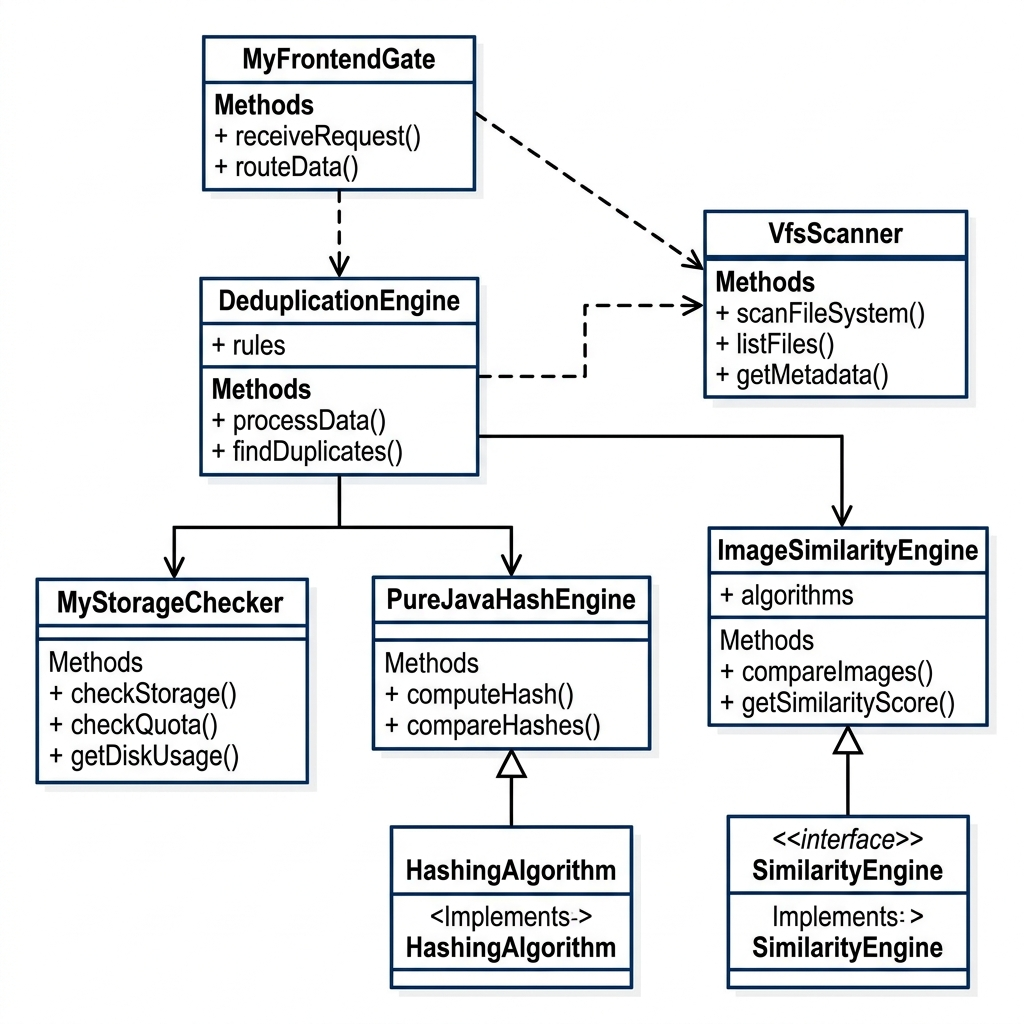
\includegraphics[width=0.8\textwidth]{images/uml_diagram.png}
    \caption{UML Class Diagram of the Deduplication Service.}
    \label{fig:uml}
\end{figure}
